\documentclass[a4paper,10pt]{article}
\usepackage[brazil]{babel}
\usepackage[utf8]{inputenc}
\usepackage[T1]{fontenc}
\usepackage{graphicx}
\usepackage{listings}
\usepackage{numprint}
\usepackage{tikz}
\usepackage[colorlinks=true,linkcolor=blue,citecolor=blue,urlcolor=blue]{hyperref}
\title {Silvver \\ Sistema de Localização por Visão VeRLab}
\author{Renato Florentino Garcia}

\usetikzlibrary{calc,3d}

% -*- latex -*-
% Definition of the Lua language for the listings package
% Time-stamp: <2008-11-30 15:27:16 rsmith>
% Written by Roland Smith <rsmith@xs4all.nl> and hereby placed in the public
% domain. 

\lstdefinelanguage{lua}
  {morekeywords={and,break,do,else,elseif,end,false,for,function,if,in,local,
     nil,not,or,repeat,return,then,true,until,while},
   morekeywords={[2]arg,assert,collectgarbage,dofile,error,_G,getfenv,
     getmetatable,ipairs,load,loadfile,loadstring,next,pairs,pcall,print,
     rawequal,rawget,rawset,select,setfenv,setmetatable,tonumber,tostring,
     type,unpack,_VERSION,xpcall},
   morekeywords={[2]coroutine.create,coroutine.resume,coroutine.running,
     coroutine.status,coroutine.wrap,coroutine.yield},
   morekeywords={[2]module,require,package.cpath,package.load,package.loaded,
     package.loaders,package.loadlib,package.path,package.preload,
     package.seeall},
   morekeywords={[2]string.byte,string.char,string.dump,string.find,
     string.format,string.gmatch,string.gsub,string.len,string.lower,
     string.match,string.rep,string.reverse,string.sub,string.upper},
   morekeywords={[2]table.concat,table.insert,table.maxn,table.remove,
   table.sort},
   morekeywords={[2]math.abs,math.acos,math.asin,math.atan,math.atan2,
     math.ceil,math.cos,math.cosh,math.deg,math.exp,math.floor,math.fmod,
     math.frexp,math.huge,math.ldexp,math.log,math.log10,math.max,math.min,
     math.modf,math.pi,math.pow,math.rad,math.random,math.randomseed,math.sin,
     math.sinh,math.sqrt,math.tan,math.tanh},
   morekeywords={[2]io.close,io.flush,io.input,io.lines,io.open,io.output,
     io.popen,io.read,io.tmpfile,io.type,io.write,file:close,file:flush,
     file:lines,file:read,file:seek,file:setvbuf,file:write},
   morekeywords={[2]os.clock,os.date,os.difftime,os.execute,os.exit,os.getenv,
     os.remove,os.rename,os.setlocale,os.time,os.tmpname},
   sensitive=true,
   morecomment=[l]{--},
   morecomment=[s]{--[[}{]]--},
   morestring=[b]",
   morestring=[d]'
  }

\lstset{numbers=left, numberstyle=\tiny, stepnumber=2, numbersep=5pt,
  basicstyle=\small\tt}

\begin{document}

\maketitle
\newpage

\tableofcontents
\newpage
\section{Introdução}
Esta documentação está desatualizada

O Silvver é um sistema que foi desenvolvido para facilitar a obtenção da
localização de alvos no ambiente. Ele possibilita que um usuário consiga de
forma transparente as localização de alvos obtidos através de vários toolkits
de localização, como por exemplo o ARToolKitPlus.

O Silvver foi construído com o objetivo de ser um sistema de localização
modular e multi-plataforma. A modularidade possibilita uma maior
escalabilidade ao sistema, cada um de seus módulos pode ser executado em uma
máquina diferente, dividindo entre elas o processamento do todo. Além disso,
os diferentes computadores podem ser espalhados espacialmente, tornando mais
fácil o uso de várias câmeras para cobrir uma grande área.

O sistema é dividido em três módulos: silvver-cameras, silvver-server e
libsilvver-client. Cada um desses módulos é um programa independente dos
demais; o silvver-cameras e o silvver-server são programas executáveis, e a
libsilvver-client é um biblioteca. Cada programa pode ser executado ou em
computadores diferentes ou na mesma máquina, e a comunicação entre eles se dá
por meio sockets.

\subsection{Silvver-cameras}

O silvver-cameras é o módulo responsável por controlar as câmeras e processar
as imagens capturadas por elas. Cada instância desse módulo pode controlar
quantas câmeras forem necessárias, e esse módulo pode ser instanciado tantas
vezes, e em quantos computadores forem necessários.

O silvver-cameras é configurado por um arquivo que descreve a cena que que
será controlada por ele. Este arquivo de configuração é um script escrito na
linguagem Lua\cite{lua}, e nele estão todas as câmeras que serão usadas e seus
parâmetros, bem como todos os tipos de alvos e suas configurações.

\subsection{Silvver-server}

O silvver-server deve ser instanciado uma única vez em todo o sistema. Ele tem
a tarefa de receber todos os alvos que foram localizados pelos vários
silvver-cameras, verificar se algum deles foi visto por mais de uma câmera ao
mesmo tempo e eliminar a duplicidade, e enviar as localizações para os
clientes interessados.

Ao ser iniciado o silvver-server passa imediatamente a ouvir uma porta TCP/IP
pré-estabelecida. A entidade ligada a esta porta é chamada recepcionista, e
todos os pedidos para adicionar ou terminar a conexão com uma câmera, e
adicionar ou retirar um cliente é recebido primeiramente por ela.


\subsection{Libsilvver-client}

A libsilvver-client é uma biblioteca C++ que fornece uma API para o acesso às
localizações de um dado alvo.

\section{Instalação}

A compilação de cada um dos módulos é feita individualmente, por serem eles
programas independentes. A única exigência quanto a bibliotecas é que a versão
da Boost\cite{boost} usada na compilação seja a mesma em todos eles, pois como
os objetos que serão enviados pela rede são serializados usando a Boost
Serialization, e versões antigas dessa biblioteca não necessariamente são
compatíveis com as serializações feitas por versões mais novas, problemas de
comunicação podem surgir.

Na raiz do projeto existem três diretórios: common, libsilvver\_client,
silvver\_cameras e silvver\_server. Em cada um dos diretórios
libsilvver\_client, silvver\_cameras e silvver\_server estão os fontes dos
respectivos módulos; já o diretório common contém os fontes que são
compartilhados entre os módulos.

Todo o projeto Silvver usa o SCons\cite{scons} como ferramenta de
compilação. Portanto, em cada uma das pastas dos módulos há um arquivo
\emph{SConstruct}, que é o script que verificas quais bibliotecas estão
instaladas no sistema, e faz a compilação e a instalação. As opções de
compilação de cada módulo podem ser vistas usando o comando \texttt{scons -h}
no mesmo diretório onde está o arquivo \emph{SConstruct}.

O processo para compilar e instalar os três módulos é excencialmente o mesmo,
por isso um mesmo exemplo pode ser seguido para todos eles, com pequenas
alterações se necessário. Dado um ambiente linux com a Boost versão 1.39
instalada em um diretório não padrão, com as bibliotecas em
\emph{/usr/local/bin} e os cabeçalhos em
\emph{/usr/local/include/boost-1\_39}. O Silvver pode ser instalado dentro do
diretório \emph{/home/renatofg/silvver} com o seguinte comando: \texttt{scons
  install --prefix=/home/renatofg/silvver/usr --lib\_boost\_suffix=-gcc43-mt-1\_39
  LIBPATH=/usr/local/lib/ CPPPATH=/usr/local/include/boost-1\_39/}.

\section{Exemplo de uso}

O primeiro módulo que dever ser executado é o silvver-server. A opção mais
importante que este ele possui é -p ou --receptionist-port, que permite
selecionar em qual porta TCP/IP o recepcionista estará ouvindo. Caso não seja
especificado, a porta 12000 será usada.

Após executado 

\section{O Arquivo de Configuração}

O arquivo de configuração do silvver-cameras é um script escrito na
linguagem de progração Lua\cite{lua}. Ao inciar o silvver-cameras criará um
ambiente lua para executar o \emph{script}, e após a execução lerá a variável
scene, que deverá ser uma tabela contento toda as estruturas necessárias.
A única variável de interesse ao silvver-cameras é a scene, todas as outras
variáveis que por ventura estejam no ambiente serão ignoradas.  Um exemplo
completo é dado abaixo:

\begin{lstlisting}[frame=lines,language=lua]
require("cameraId")
require("cameraConstructors")

scene = {
    cameras = {
        Dragonfly{
            uid = dragonfly2uid(5110432),

            focal_length = {531.20605, 531.45104},
            principal_point = {359.2638, 278.30819},
            radial_coef = {-0.43208, 0.236, 0},
            tangential_coef = {-0.00054004, 0.003849},

            translation_vector = {358.43, -2.3797, 921.3742},
            rotation_matrix = {
                0.9960135, 0.0050411, -0.0890,
                0.0013316, -0.99913, -0.04166,
                    -0.08919, 0.04137, -0.99515
            },

            shutter = 500,
            gain = 800,
            white_balance = {50, 5},
        },
    },

    artp_targets = {

        pattern_width = 150,

        {
            pattern_file = 'data/4x4patt/4x4_1.patt',
            uid = 1,
        },
    },
}
\end{lstlisting}

As linhas 1 e 2 incluem dois fontes com funções que implementam algumas
facilidades. Cada câmera possui um número que a identifica univocamente (UID),
e dependendo da biblioteca utilizada, como a libdc1394, esse número difere do
UID dado pelo fabricante. Em camedaId estão funções que traduzem os
identificadores dados pelo fabricante da câmera para o UID esperado pela
biblioteca. Esse é o caso de dragonfly2uid, que recebe o UID no formato dado
nas câmeras dragonfly e retorna um UID no formato esperado pela libdc1394.

Cada câmera possui diversas opções de configuração, e para que não seja
necessário especificar cada um desses parâmetros.

\section{Calibração das Câmeras}

O processo de calibração de uma câmera consiste de se procurar os melhores
parâmetros para um modelo teórico que a descreva através de equações
matemáticas, sendo que estes parâmetros podem ser divididos entre intrínsecos
e extrínsecos. Os parâmetros intrínsecos definem as características opticas,
geométricas e digitais da câmera. No Silvver, os parâmetros intrínsecos de
interesse são: distância focal, ponto principal, três parâmetros de distorção
radial e dois parâmetros de distorção tangencial. Os parâmetros extrínsecos
por sua vez descrevem como a câmera está posicionada no mundo, através de um
vetor de deslocamento e uma matriz de rotação é dada a pose da câmera em
relação a uma origem no mundo.

Dois scripts para a calibração de câmeras fazem parte do projeto Silvver, são
eles \emph{silvverIntCalib} e \emph{silvverExtCalib}, que são usados para
determinar os parâmetros intrínsecos e extrínsecos respectivamente.

\subsection{SilvverIntCalib}

\begin{figure}
  \centering
  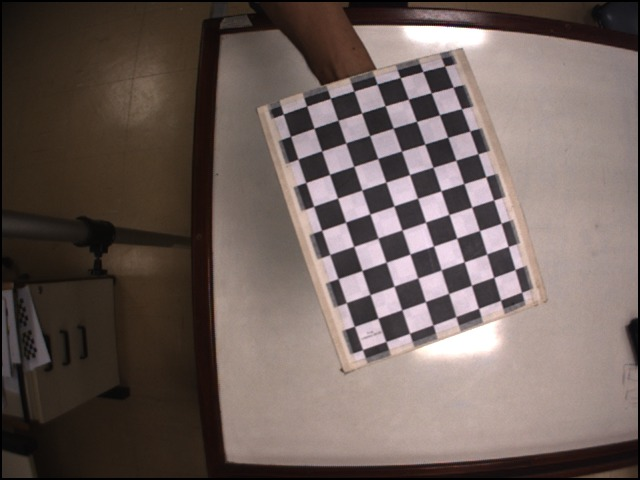
\includegraphics[width=0.5\columnwidth]{figures/checkerboard}
  \caption{Exemplo de imagem usada para a calibração intrínseca de uma
    câmera.}
  \label{fig:checkerboard}
\end{figure}

A calibração intrínseca usando o script \emph{silvverIntCalib} é feita por
meio de imagens de um tabuleiro xadrez capturadas pela câmera em questão, como
a imagem da figura \ref{fig:checkerboard}. O primeiro passo portanto para a
calibração intrínseca é salvar uma sequência de imagens em que seja possível
ver completamente um tabuleiro. Uma vez que se tenha as imagens, basta
executar o script passando-as como argumento.

Assumindo-se que se esteja no mesmo diretório que as imagens, todas elas com
extensão .ppm; e o tabuleiro seja o mesmo da figura \ref{fig:checkerboard},
com 10$\times$7 casas, e cada casa medindo \numprint[mm]{25}, a calibração
poderia ser obtida com o seguinte comando: \texttt{silvverIntCalib 10 7 0.025
  *.ppm}. O silvverIntCalib também aceita algumas opções, que podem ser vistas
pelo comando \texttt{silvverIntCalib -h}.

\subsection{SilvverExtCalib}

\begin{figure}[h]
  \centering
  \begin{tikzpicture}
    \draw (0,0,0) -- (1,0,0);
    \draw (0,0,0) -- (0,1,0);
    \draw (0,0,0) -- (0,0,1);
  \end{tikzpicture}
  \caption{oi}
  \label{fig:silvverExtCalib}
\end{figure}

O problema da calibração extrínseca resolvido pelo silvverExtCalib é definido
pelo seguinte enunciado: em um espaço tridimensional, seja uma pose
$\mathrm{P_1}$ e uma câmera C. São conhecidas as coordenadas (x, y, z, e a
matriz de rotação) da pose $\mathrm{P_1}$ em relação a uma origem O
($\mathrm{P_1^O}$), e em relação à camera C ($\mathrm{P_1^C}$). Deseja-se
obter a pose da camera C em relação à origem O ($\mathrm{P_C^O}$). Ou seja,
tendo-se $\mathrm{P_1^O}$ e $\mathrm{P_1^C}$ deseja-se conhecer
$\mathrm{P_C^O}$, como está ilustrado na figura \ref{fig:silvverExtCalib}. O
que o silvverExtCalib faz é essa transformação vetorial.


Uma forma prática se obter $\mathrm{P_1^O}$ e $\mathrm{P_1^C}$, ambos
pré-requisitos no processo de calibração, é utilizando um alvo para o qual o
Silvver forneça uma pose 6D. Vamos assumir que a pose desse alvo seja
$\mathrm{P_1}$. Caso se deseje que $\mathrm{P_1}$ corresponda à origem do mundo, para
determinar $\mathrm{P_1^O}$ basta fazer $(x,y,z) = (0,0,0)$ e a matriz de
rotação igual à matriz identidade. Caso $\mathrm{P_1}$ não esteja na origem do
mundo, sua pose $\mathrm{P_1^O}$ pode ser dada usando o Silvver e uma segunda
câmera já calibrada.

Para encontrar $\mathrm{P_1^C}$ basta configurar o silvver-cameras tendo a
câmera C na origem do mundo, e obter a localização de $\mathrm{P_1}$. Para
isso, o arquivo de configuração lua teria o seguinte trecho de código na
tabela referente à camera C:
\begin{lstlisting}[numbers=none]
    translation_vector = {0, 0, 0},
    rotation_matrix = {
        1, 0, 0,
        0, 1, 0,
        0, 0, 1},
\end{lstlisting}

O formato de entrada de $\mathrm{P_1^O}$ e $\mathrm{P_1^C}$ esperado pelo
silvverExtCalib é um arquivo de texto para cada uma, dentro do qual está sua
pose. Se $\mathrm{P_1^O}$ e/ou $\mathrm{P_1^C}$ foram obtidas usando o
Silvver, possivelmente seu arquivo de texto correspondente é formado por
várias linhas, onde cada uma delas é a localização de $\mathrm{P_1}$ em um
dado instante de tempo. Neste caso o silvverExtCalib tomará a média desses
valores como a pose que será utilizada.

Tendo-se $\mathrm{P_1^O}$ em um arquivo de texto nomeado \emph{p1o.txt}, e
$\mathrm{P_1^C}$ em um nomeado \emph{p1c.txt}, para encontrar $\mathrm{P_C^O}$
basta executar o seguinte comando estando-se no mesmo mesmo diretório em que
estão os arquivos \emph{p1o.txt} e \emph{p1c.txt}: \texttt{silvverExtCalib
  p1o.txt p1c.txt}.

\section{Desenvolvimento}

Durante a construção do projeto Silvver foi tomado um cuidado durante o
um desenho das classes, tal que permitisse que se adicionasse novos modelos de
câmeras e de marcos de uma maneira simples dentro do possível. Nesta seção
será feito um exemplo passo-a-passo de como é esse processo de acrescentar
suporte a mais uma câmera e mais um tipo de marco.

\subsection{Adicionando uma nova classe de câmeras}

\begin{figure}[h!]
  \centering
  \includegraphics[width=0.5\columnwidth]{figures/pinholeSpam}
  \caption{Pinhole Spam camera}
  \label{fig:pinholeSpam}
\end{figure}

Vamos supor que o Silvver já trabalhe com pseudo câmeras e câmeras que sejam
acessadas pela biblioteca libdc1394, e que desejamos adicionar suporte para
que uma pinhole Spam câmera (figura \ref{fig:pinholeSpam}) possa também ser
usada. Como o módulo silvver-camera é o único que acesssa diretamente as
câmeras, somente ele deverá ser alterado para que as Spam câmeras se integrem
ao sistema. Também por esse motivo, para facilitar a leitura no restante dessa
subseção, quando o nome de um arquivo for dado, seu caminho será referente à pasta
\emph{silvver\_cameras/src/}, exceto quando explícito o caminho completo.

\subsubsection{Alterações nos fontes do projeto}
O primeiro passo para que o Silvver funcione com as câmeras Spam é criar uma
struct que conterá todas as opções e configurações necessárias para a
inicialização da Spam câmera. Essa struct deverá ficar dentro do cabeçalho
\emph{hardCameras/hardCameraDescriptions.hpp}. Neste mesmo arquivo há uma
struct chamada \emph{Hardware}, na qual estão todas as opções comuns a todos
os tipos de câmeras. Portanto, a nova struct que será criada deverá derivar
publicamente da struct \emph{Hardware}. O código poderia ser:
\begin{lstlisting}[frame=lines,language=c++]
struct Spam :public Hardware
{
  std::string devicePath;

  float holeSize;
};
\end{lstlisting}
Além disso, no cabeçalho \emph{hardCameras/hardCameraDescriptions.hpp} há um
typedef chamado\emph{AnyHardwareCamera}, o qual consiste de um \emph{boost
  variant} que abarca todas as structs com configuração das câmeras. Portanto,
a nova struct deve ser colocada neste variant, que ficaria assim:
\begin{lstlisting}[frame=lines,language=c++]
typedef boost::variant<PseudoCamera,
                       DC1394,
                       Spam         > AnyHardwareCamera;
\end{lstlisting}

O próxima passo é escrever o código que irá criar a struct \emph{Spam} de
acordo com as opções dadas no arquivo de configuração lua. A leitura do
arquivo de configuração é feito pela classe \emph{CfParser}, que é declarada
em \emph{cfParser.hpp} e definida em \emph{cfParser.cpp}. A única alteração
necessária em \emph{cfParser.hpp} será a declaração do método privado que lerá
as configurações. Esse método deverá retornar uma struct \emph{Spam}, e recebe
um apontador para um \emph{lua\_State} como argumento. Neste exemplo essa
declaração seria:
\begin{lstlisting}[frame=lines,language=c++]
scene::Spam readSpamConfig(lua_State* L);
\end{lstlisting}
Já em \emph{cfParser.cpp}, primeiramente o método \emph{readCamera} deverá ser
alterado, para que o método recém criado \emph{readSpamConfig} seja chamado
quando apropriado. Como o que define qual o tipo de câmera está sendo descrito
em uma dada tabela lua do arquivo de configuração é o campo \emph{\_\_driver}, o
código que deveria ser adicionado no método \emph{readCamera} seria:
\begin{lstlisting}[frame=lines,language=c++]
else if (driver == "spam")
{
  camera.hardware = this->readSpamConfig(L);
}
\end{lstlisting}
E finalmente, o método \emph{readSpamConfig} poderia ser definido como se segue:
\begin{lstlisting}[frame=lines,language=c++]
scene::Spam
CfParser::readSpamConfig(lua_State* L)
{
  scene::Spam spam;

  spam.devicePath = readValue<std::string>(L, "device_path");
  spam.holeSize   = readValue<float>(L, "hole_size");
  this->readHardware(L, spam);

  return spam;
}
\end{lstlisting}
Logicamente, os nomes \emph{device\_path} e \emph{hole\_size}, devem
corresponder aos nomes dados no arquivo de configuração.

A criação das instâncias das classes que controlam as hardCameras é feita pela
classe \emph{HardCameraFactory}. Para que a nova classe possa ser construida,
é necessário também colocá-la na factory. No cabeçalho
\emph{hardCameraFactory.hpp} a alteração se resume a adicionar um método à
struct \emph{ConstructHardCamera}. Este é o método que instanciará uma spam
câmera, e com adição já feita, o código seria:
\begin{lstlisting}[frame=lines,language=c++]
struct ConstructHardCamera
  :public boost::static_visitor<HardCamera*>
{
  HardCamera* operator()(const scene::PseudoCamera& config) const;
  HardCamera* operator()(const scene::DC1394& config) const;
  HardCamera* operator()(const scene::Spam& config) const;
};
\end{lstlisting}
Como o suporte a Spam câmeras não é um requerimento necessário para o
funcionamento do Silvver, pode-se optar por não compilar a classe que está
sendo presentemente desenvolvida. A indicação de que o silvver-camera deve ser
compilado com suporte a Spam câmeras é dado pela macro HAVE\_SPAM\_H, e
portanto, no fonte \emph{hardCameraFactory.cpp} a inclusão do cabeçalho
\emph{spam.hpp} deve estar entre include guards como se segue:
\begin{lstlisting}[frame=lines,language=c++]
#ifdef HAVE_SPAM_H
#  include "hardCameras/spam.hpp"
#endif
\end{lstlisting}
A definição do método \emph{operator()(const scene::Spam\& config) const} pode
ser como se segue:
\begin{lstlisting}[frame=lines,language=c++]
HardCamera*
HardCameraFactory::ConstructHardCamera::
  operator()(const scene::Spam& config) const
{
#ifdef HAVE_SPAM_H
  return (new Spam(config));
#else
  throw std::invalid_argument(``This program dont was ``\
                              ``compiled with support ``\
                              ``to spam cameras'');
#endif
}
\end{lstlisting}

\subsubsection{A classe Spam}
A classe Spam que controlará as câmeras Spam deverá obedecer algumas
exigências. Primeiramente, seus arquivos fonte deverão estar dentro da pasta
\emph{hardCameras}, por exemplo \emph{hardCameras/spam.hpp} e
\emph{hardCameras/spam.cpp}.

A relação entre as câmeras e as classes que localizam os marcos obedecem à
lógica descrita pelo design pattern observer, tendo um papel como
subject. Todo o protocolo do pattern é implementado pela classe base abstrata
HardCamera, a responsabilidade das classes que efetivamente controlarão as
câmeras é continuamente capturar imagens e disponibilizá-las aos observers
usando as as facilidades da classe base HardCameras.

Dado o exposto, a classe \emph{Spam} deverá herdar publicamente da classe
\emph{HardCamera}. Ela deverá implementar o método abstrato initialize, onde a
câmera deverá ser inicializada, e ao final do qual deverá ser lançada uma nova
thread onde o método a ser executado irá capturar as imagens continuamente.



ao final do qual a câmera deverá estar funcionando.

\subsubsection{Alteração dos arquivos SCons}
Como último passo, deve-se acrescentar as instruções para que o
SCons\cite{scons} adicione as novas opções de compilação apropriadas e compile
o projeto. Dois arquivos são relevantes neste passo:
\emph{silvver\_cameras/SConstruct} e
\emph{silvver\_cameras/src/SConscript}. Os dois servem como entrada para o
SCons, e contém toda a informação sobre o programa que será construído, eles
são escritos em linguagem Python. Vamos supor neste exemplo que para acessar
as câmeras Spam exista uma biblioteca \emph{spam} com uma API dada em
\emph{spam.h}.

No arquivo \emph{silvver\_cameras/SConstruct} há uma variável chamada
camera\_libs que é um dicionário contendo informações sobre todas as
bibliotecas externas que são usadas para controlar câmeras. Nós deveremos
adicionar uma instância da classe Library (classe definida em
\emph{common/sconsUtilities.py}. O construtor dessa classe aceita os seguintes
argumentos, fora de ordem:
\begin{itemize}
\item name O nome da biblioteca
\item short\_name Um nome simplificado para ser usado nas opções de linha de comando
\item headers Os cabeçalhos da biblioteca
\item libraries As libs da biblioteca
\end{itemize}
O código seria o seguinte:
\begin{lstlisting}[frame=lines,language=python]
camera_libs['spam'] = Library(name='Spam',
                              headers=['spam.h'],
                              libs=['spam'])
camera_libs['spam].description = 'Spam pinhole cameras'
\end{lstlisting}
A variável description possui o texto que será usado quando forem listadas
as câmeras com as quais o silvver-camera funcionará quando for compilado.

No arquivo \emph{silvver\_cameras/src/SConscript} deverá ser testado se a
biblioteca Spam foi encontrada no sistema, e em caso positivo adicionar o
fonte \emph{hardCameras/spam.cpp} à lista de arquivos que serão compilados, e
definir a macro HAVE\_SPAM\_H necessária para que o código seja corretamente
compilado. O código seria:
\begin{lstlisting}[frame=lines,language=python]
if cleaning or camera_libs['spam']:
    env.Append(CXXFLAGS = '-DHAVE_SPAM_H')
    sources += ['hardCameras/spam.cpp']
\end{lstlisting}
O teste da variável cleaning deve ser feito, caso contrário o código objeto
gerado na compilação de spam.cpp não será deletado quando se executa o SCons
com o parâmetro -c.

\subsubsection{Alteração dos arquivos Lua}
No arquivo \emph{silvver\_cameras/lua/cameraConstructor.lua} ficam funções que
facilitam a descrição das câmeras no arquivo de configuração Lua, por exemplo
colocando valores default para os campos que forem omitidos. As funções podem
ser referente a um modelo de câmera específico, ou a toda uma classe de
câmeras.


\bibliography{silvver}
\bibliographystyle{plain}

\end{document}
